\chapter{语句级的情感分析模型}
\section{知识模型}
基于Stanford Parser的知识模型主要使用语法特征和情感词典对文本进行情感分类,该方法不需要训练,处理短文本时速度较快,适合处理情感较为强烈,使用情感词较多,逻辑较为简单的语句。
\subsection{Stanford 语法树}
Stanford Parser是由斯坦福自然语言处理小组实现的语法分析工具,也是Stanford CoreNLP的其中一个组件。它主要基于概率上下文无关文法(Probabilistic Context Free Grammar,PCFG,又称随机上下文无关文法,Stochastic Context Free Grammar,SCFG),能进行句法分析和语义依存分析(Semantic Dependency Parsing, SDP),生成语法树和依赖关系,是目前比较主流的一款语法分析工具。\par
本文选择Stanford Parser作为句法分析器,因此在此简单介绍Stanford Parser的中心算法思想。\par

定义:一个概率上下文无关文法是一个五元组($N,\Sigma ,S,R,P$),其中$N$为非终结符集,$\Sigma$为终结符集,$S\in N$为开始符集,$R$为产生式集,对于任意产生式$r \in R$,其概率为$P(r)$。规则表示形式为:$A\rightarrow\alpha$,其中$A$为非终结符,$p$为$A$推导出$\alpha$的概率,即$p = P(A\rightarrow\alpha)$,该概率分布必须满足如下条件:$\sum{P(A\rightarrow\alpha)}=1$
\cite{Cha93}\par
对应于语法树,$N$相当于非叶节点,$\Sigma$为叶节点,$S$唯一且$S$为根节点,$R$为可行的路径,$P$为使用某条路径转移的概率。\par
在实践中,$P(A\rightarrow\alpha)$一般设为训练集语料中$A\rightarrow\alpha$的最大似然估计,也即$P(A\rightarrow\alpha) = \frac{Count(A\rightarrow\alpha)}{Count(A)}$,其中$Count(A\rightarrow\alpha)$为已标注语料中出现该规则的次数,$Count(A)$为语料中出现该语法单元的次数。给定语法树后,就能计算出已标注词性的文本符合语法树的概率,而寻找对应的语法树可以转化为动态规划问题求解。\par
明显,PCFG是CFG(上下文无关算法)的拓展,但上下文算法不含概率,无法解决语言的二义性问题,因此PCFG要比CFG更适合于自然语言处理。\par
但由于PCFG等价地对待词组中的所有词,导致相同结构的PCFG对词汇信息和结构偏向不明显。词汇化的PCFG文法为每个语法树的每个节点添加首要词(HEAD),从而克服了PCFG文法的弱点,取得了巨大的成功\cite{Klein2003b}。\par
本文使用Factor模型,在Stanford Parser Factor模型中词汇化的PCFG方法用于同时表示语法结构与依赖关系,如图\ref{parser1}c。Klien等\cite{Klein2003a} 人认为,设$L$为词汇化的PCFG树,则$L$可以被一棵语法PCFG树$T$(如图\ref{parser1}a)和一棵结构相符合的依赖关系树$D$(如图\ref{parser1}b)确定。于是,基于文本构建$L$的问题就被转化为基于文本构建一对$T$,$D$,使$P'(T,D)$最大,这里$P'(T,D)$代表文本同时符合$T$,$D$的概率。Klein等人进一步假设$T$与$D$相对独立,也即$P'(T,D) = P'(T)P'(D)$,并分别使用动态规划构建概率最大的$T$,$D$,之后使用A*启发式算法搜索T和D的近似结合方式,该算法取得了不错的成果。\par
Stanford Parser还对分析器做了一系列优化\cite{LevyM03} \cite{Marneffe06} \cite{Zhang2011} \cite{ChenM14} \cite{SocherBMN13} \cite{Nivre16} \cite{SchusterM16},在此不做赘述。
\begin{figure}
\begin{center}
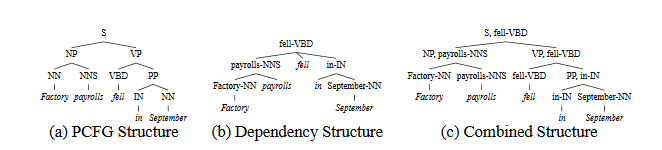
\includegraphics[width=\textwidth]{graphic/parser1.PNG}
\caption{三种分析结构 \label{parser1}}
\end{center}
\end{figure}
\subsection{基本流程}
算法基本流程如图\ref{plainmodel1}\par
\begin{figure}
\begin{center}
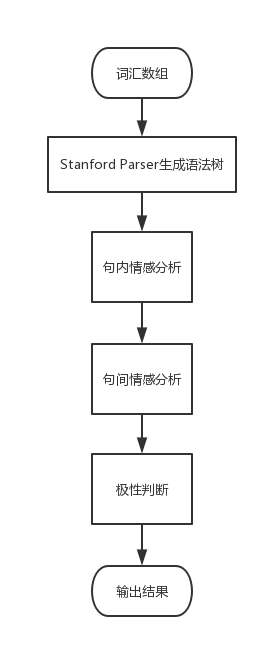
\includegraphics {graphic/plainmodel1.png}
\caption{知识模型基本流程图 \label{plainmodel1}}
\end{center}
\end{figure}
伪代码如下:\par
\lstset{language=python}
\begin{lstlisting}
def analyze(words, lang):
  if lang == 'zh':
    trees = parser_zh.parse(words)
  else:
    trees = parser_en.parse(words)
  ans = 0
  for tree in trees:
    dfs(tree.root,tree)
    ans += tree.root.sentiment
  return ans

def dfs(node, tree):
  node.phrase = ''
  if not isleaf(node):
    for child in node.daughterTrees:
      dfs(child, tree)
  if isleaf(node):
    node.phrase = node.label
  else:
      for child in node.daughterTrees:
        if lang == 'zh':
          node.phrase = node.phrase + child.phrase
        else:
          if isW(child) or child.label == "n't":
            node.phrase = node.phrase + child.phrase
          else:
            node.phrase = node.phrase + ' ' + child.phrase
  found, node.sentiment = lookup_in_emotion(node.phrase)
  if not found:
    found, node.sentiment = lookup_in_degree(node.phrase)
  if not found:
    if not isleaf(node):
      d = 0
      e = 0
      for child in daughterTrees:
        if child.label == 'RB'
          or child.label == 'AD':
          d += child.sentiment
        else:
          e += child.sentiment
      if d == 0:
        node.sentiment = e
      elif e == 0:
        node.sentiment = d
      else:
        node.sentiment = d * e
\end{lstlisting}
算法首先将分词后的词汇输入到Stanford Parser中,每个短句将生成一棵独立的语法树。\par
接着算法对每个短句所生成的语法树采用top-down递归遍历。\par
本文主要使用两个词典,一个为情感词典emotion,另一个为程度词典degree。\par
在递归的过程中,算法会首先在词典中查找子树所对应的短语,如果找到了对应的短语,则将短语所代表的情感强度或者程度强度设为该子树的强度,否则,分别统计子树的子节点的情感强度和程度强度,取其乘积作为该子树的强度。\par
最后,算法将多棵语法树根节点的情感强度相加,得到整体情感强度。\par
如图,对于“This is the right size for any use!  Uses little space and looks extremely good on the counter.”,Stanford Parser将会生成以下结果,可视化后相当于图\ref{fig:plainf2}和\ref{fig:plainf3}:\par

\begin{lstlisting}
(ROOT
  (S
    (NP (DT This))
    (VP (VBZ is)
      (NP
        (NP (DT the) (JJ right) (NN size))
        (PP (IN for)
          (NP (DT any) (NN use)))))
    (. !)))

(ROOT
  (S
    (VP
      (VP (VB Uses)
        (NP (JJ little) (NN space)))
      (CC and)
      (VP (VBZ looks)
        (ADJP (RB extremely) (JJ good))
        (PP (IN on)
          (NP (DT the) (NN counter)))))
    (. .)))
\end{lstlisting}

\begin{center}
\begin{figure}
\subfigure[语法树]{
	\label{fig:plainf2}
	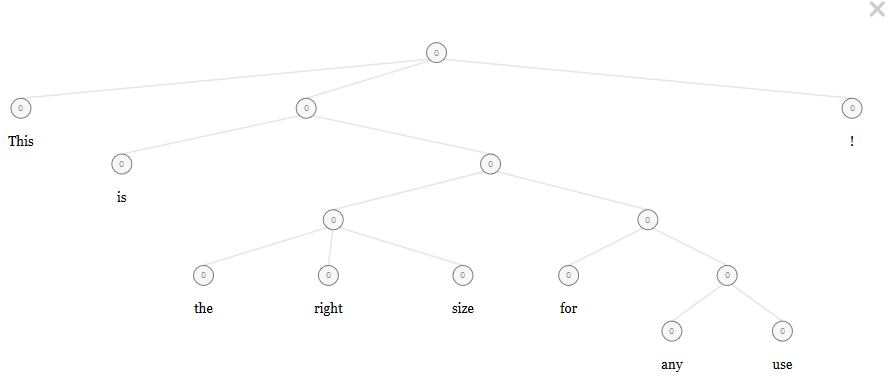
\includegraphics[width=0.8\textwidth]{graphic/plainmodel2.png}
}
\subfigure[语法树]{
	\label{fig:plainf3}
	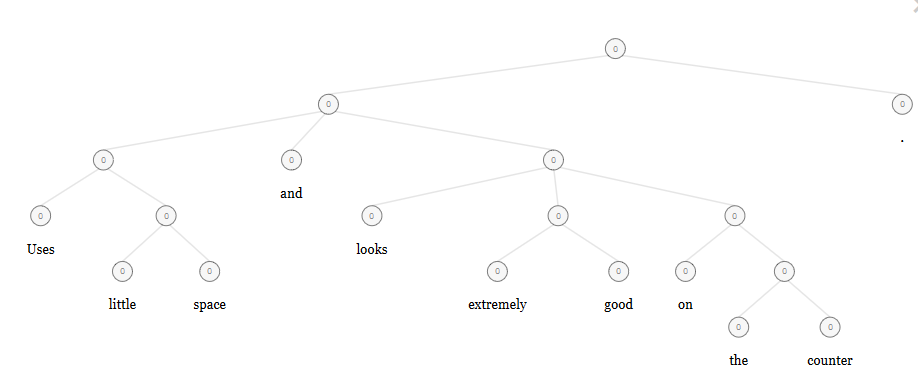
\includegraphics[width=0.8\textwidth]{graphic/plainmodel3.png}
}
\end{figure}
\end{center}

算法分别从左右两棵树根节点开始分析,逐步到达叶节点,以右边的树为例,该树对应"Uses little space and looks extremely good on the counter."。\par
\begin{enumerate}

\item 在情感词典中,"little"的情感强度为-1.0,因此"little space","Use little space"的情感强度都被标注为-1.0。
\item "extremely"在程度词典中被标注为+2.0,"good"在情感词典中被标注为+1.0,因此"extremely good", "looks extremely good on the counter."被标注为+2.0
\item 综上,"Uses little space and looks extremely good on the counter."被标注为+1.0
\item 右边的树也遵循此流程,极性为+1.0,将子句合并考虑,得到该语句整体情感强度为+2.0。
\end{enumerate}\par
最终,算法结果可视化如图\ref{fig:plainf4} \ref{fig:plainf5}。

\begin{center}
\begin{figure}
\subfigure[知识模型结果可视化]{
	\label{fig:plainf4}
	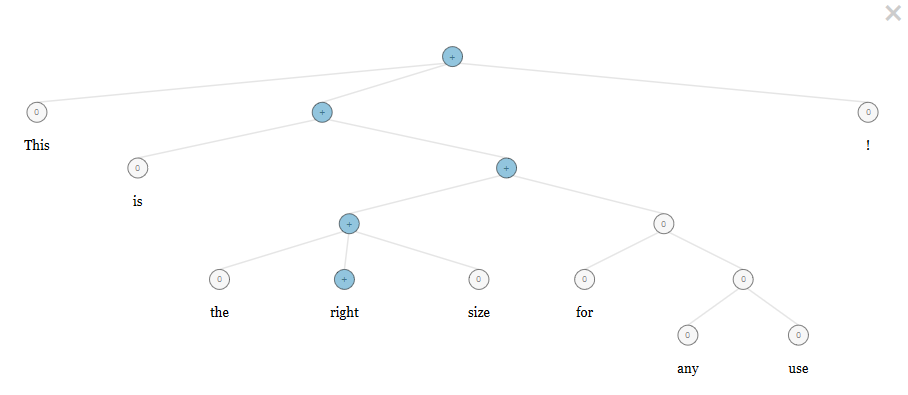
\includegraphics[width=0.8\textwidth]{graphic/plainmodel4.png}
}
\subfigure[知识模型结果可视化]{
	\label{fig:plainf5}
	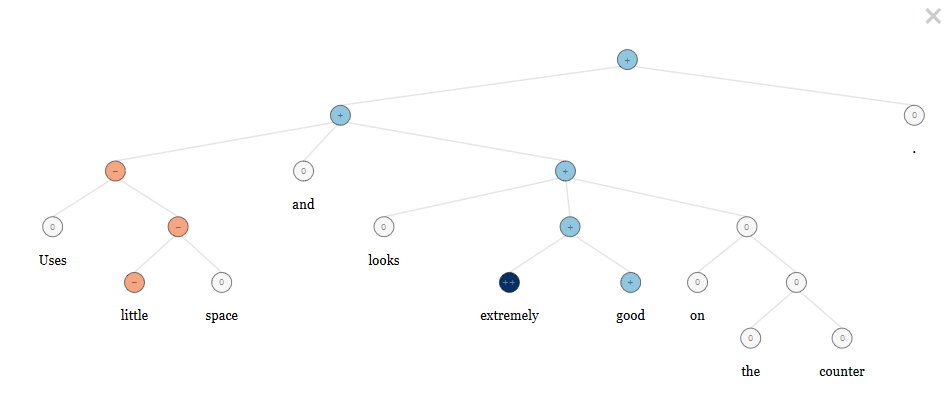
\includegraphics[width=0.8\textwidth]{graphic/plainmodel5.png}
}
\end{figure}
\end{center}

\section{深度学习相关算法}
本节将从人工神经网络(Artificial Neural Networks, ANN)开始,分别简单介绍反向传播网络(Back Propagation, BP),卷积神经网络(Convolutional Neural Networks, CNN),循环神经网络(Recurrent Neural Networks, RNN),长短时记忆型循环神经网络(Long Short Term Memory, LSTM),优化算法等模型中可能用到的相关算法。
\subsection{人工神经网络}
人工神经网络提供了一种普遍且实用的方法从样例中学习值为实数,离散值或向量。ANN在一定程度上受到生物大脑中神经元相互连接的模型的启发,它由许多基本单元构成,每个单元有一定的实值输入(该输入可能来自外部也可能是其它单元的输出),同时产生单一的实数值输出。常见ANN的基本单元如图\ref{ann1}:
\begin{figure}[!hbp]
\begin{center}
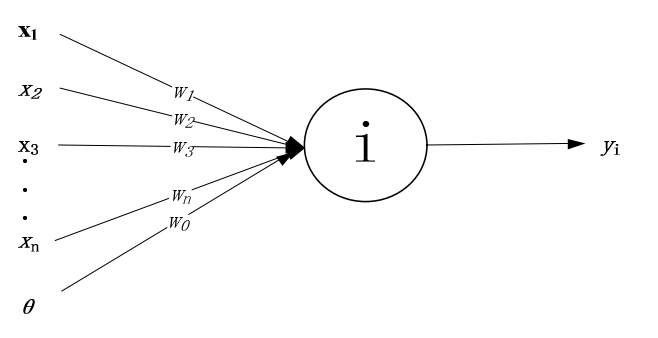
\includegraphics[width=0.4\textwidth]{graphic/ann1.png}
\caption{ANN基本单元\cite{ml2006} \label{ann1}}
\end{center}
\end{figure}
其函数可以写作
\begin{equation}
o(\vec{x}) = f(\vec{w} \vec{x} - b)
\end{equation}
其中$\vec{x}$为输入,$f$为激活函数,负责将线性输出转变为非线性输出以增加神经网络的表达能力,$\vec{w}$为权重(weights),$b$为偏置(bias),与$\vec{w} \vec{x} $具有相同形状。$\vec{w}$与$b$通常是神经网络训练的主要对象。
常用的激活函数有sigmoid(又称logistic函数),tanh,ReLu(Rectified Linear Unit)等,具体公式如下:
\begin{center}
\begin{tabu}  to 0.8\textwidth{X|X[3]|X[3]}
\hline
函数名称 & 函数 & 导数 \\
\hline
sigmoid &
$$
f(y) = \frac{1}{1 + e^{-y}}
$$
&
$$
\frac{df(y)}{dy} = f(y) \times (1 - f(y))
$$
\\ \hline
tanh &
$$
f(y) = tanh(y) = \frac{e^x - e^{-x}}{e^x + e^{-x}}
$$
&
$$
\frac{df(y)}{dy} = 1 - {f(y)}^2
$$
\\ \hline
ReLU &
$$
f(y) = \left\{\begin{matrix}
y & if\ y > 0\\ 
0 & if\ y \leq 0
\end{matrix}\right.
$$
&
$$
\frac{df(y)}{y} = \left\{\begin{matrix}
1 & if\ y > 0\\ 
0 & if\ y \leq 0
\end{matrix}\right.
$$
\\ \hline
\end{tabu}
\end{center}
由于sigmoid函数和tan函数的导数是线性输出的二次多项式,在训练时易导致梯度爆炸或梯度消失问题,故本文中线性层之间的激活函数主要选用ReLU函数。\par
一个较典型的人工神经网络通常由多层基本单元构成,如图\ref{ann2},通常有输入层,隐含层,输出层,各层之间通过激活函数将线性输出转化为非线性输出。\par

\begin{figure}[!hbp]
\begin{center}
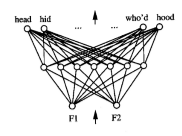
\includegraphics[width=0.4\textwidth]{graphic/ann2.png}
\caption{典型ANN结构\cite{ml2006} \label{ann2}}
\end{center}
\end{figure}

\subsection{损失计算函数}
本文中主要使用带有softmax的交叉熵函数计算网络输出值和目标值之间的误差。softmax函数是sigmoid函数在多分类问题上的拓展。
\begin{equation}
softmax(t_i) = \frac{e^{t_i}}{\sum_j{e^{t_j}}}
\end{equation}
其中$\vec{t}$为网络的输出,其长度为类别总数。
\begin{equation}
loss = crossentropy(\vec{S}, \vec{L}) 
= \sum_i {(L_i * log(s_i))}, \vec{S} = softmax{(\vec{t})}
\end{equation}
其中$\vec{L}$为网络的目标值,其长度为类别总数。

\subsection{反向传播网络}
反向传播算法是目前多层神经网络主要的训练方法,它主要基于微积分的链式求导法则\ref{chainrule},对神经网络从输出层向上进行快速求导。

\begin{equation} \label{chainrule}
(f(g(y)))' = f'(g(y)) * g'(y)
\end{equation}
反向传播神经网络的训练基本流程是:\par
\begin{enumerate}
\item 初始化网络
\item 首先将输入沿前向传播,求出误差
\item 使误差沿网络反向传播,计算梯度,从而使用优化方法更新权值。
\item 如果达到终止条件,跳出循环,否则,重复第2-4步。
\end{enumerate}

\subsection{优化方法}
在神经网络上训练时,其假设空间为所有可能的实数权向量的集合(将偏置等参数也视为权向量),一个高维空间。当误差函数和目标值已知时,假设空间中会形成一个误差曲面,而训练的目的就是尽可能找到该误差曲面的最小值。\par
如图\ref{ann3}是二维假设空间中误差曲面的假想图,可以看出该误差曲面是具有单一全局最小值的抛物面,沿梯度方向可以到达该最小值点。\par
\begin{figure}[!hbp]
\begin{center}
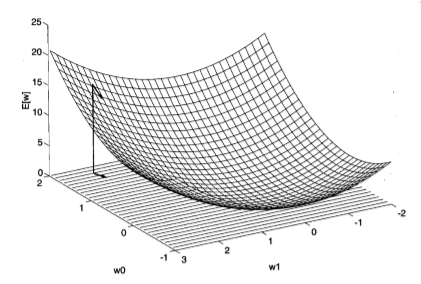
\includegraphics[width=0.4\textwidth]{graphic/ann3.png}
\caption{误差曲面\cite{ml2006} \label{ann3}}
\end{center}
\end{figure}
\subsubsection{随机梯度下降方法}
为了确定一个使误差最小化的权向量,梯度下降搜索从初始权向量出发,每一步都沿梯度方向修改该权向量,直到到达全局最小误差点。\par
该训练法则可以写为:\cite{ml2006}
\begin{equation}
w_i \leftarrow w_i + \eta\Delta w_i
\end{equation}
其中$\Delta w_i$为误差相对于分量$w_i$方向上的梯度,$\eta$为控制步长的学习速率。\par
但梯度下降方法每一步都需要计算所有训练样例上的整体误差,同时,梯度下降方法很可能收敛到局部极小值。\par
为了缓解这些困难,人们提出了随机梯度下降算法,该算法根据每个训练样例batch单独计算误差来更新权值,相当于为每个batch单独定义不同的误差函数。因此,如果误差平面上有多个局部极小值,随机梯度下降算法可以通过不同的误差避免陷入局部最小值。
\subsubsection{Adagrad方法}
虽然随机梯度下降方法为避免陷入局部最小值提供了可行的方法,但梯度下降方法对所有需要更新的权向量都使用了全局学习速率,而全局学习速率可能不适应于所有的参数。Adagrad(Adaptive Subgradient)方法\cite{adagrad}能够对每个参数自适应不同的学习速率,对稀疏特征使用更大的学习速率,因此更适应于处理稀疏数据。\par
其学习速率为:
\begin{equation}
\eta_{t, i} = \frac{\eta_0}{ \sqrt{\sum_{j=1}^{t}{G_{j,i}^2} + \epsilon}}
\end{equation}
其中,$\eta_{t, i}$为t时刻对于权重$w_i$的学习速率,$\eta_0$为初始学习速率,$\epsilon$为平滑常数,用于防止分母为0,$G_{j,i}$代表j时刻$w_i$方向上的梯度。

\subsubsection{ADADELTA方法}
Zeiler等\cite{adadelta}人认为Adagrad方法存在三个问题:
\begin{enumerate}
\item 其学习率单调递减,训练后期学习率过小。
\item 需要手工设置一个全局的初始学习率。
\item 更新$X_t$时存在单位不统一现象。
\end{enumerate}
因此Zeiler等人提出了ADADELTA方法,用于改进Adagrad方法。ADADELTA算法基于牛顿迭代法,其学习速率不再基于全部梯度平方之和,而主要基于最近的梯度。
其学习速率更新规则为:
\begin{equation}
E[g^2]_t = \rho E[g^2]_{t-1} + (1-\rho )g_t^2
\end{equation}
\begin{equation}
\eta_t =  -\frac{\sqrt{E[\eta^2]_{t-1} + \epsilon}}{\sqrt{E[g^2]_{t} + \epsilon}}g_t
\end{equation}
\begin{equation}
E[\eta^2]_t = \rho E[\eta^2]_{t-1} + (1-\rho )\eta_t^2
\end{equation}
其中$g_t$为t时刻的梯度,$\rho$为衰减速率,$\epsilon$为平滑常数。

\subsubsection{ADAM方法}
ADAM(Adaptive Moment Estimation)\cite{adam}根据损失函数对每个参数的梯度的一阶矩估计和二阶矩估计动态调整针对于每个参数的学习速率,其中一阶矩的作用类似于冲量项(momentum),二阶矩则与ADADELTA算法相似。ADAM算法迭代更新步长有一个较为稳定的范围,因此更适合RNN。

\begin{equation}
m_t = \beta_1 m_{t - 1} + (1 - \beta_1)g_t
\end{equation}
\begin{equation}
v_t = \beta_2 m_{t - 1} + (1 - \beta_2)g_t^2
\end{equation}
\begin{equation}
\hat{m_t} = \frac{m_t}{1 - \beta_1^t}
\end{equation}
\begin{equation}
\hat{v_t} = \frac{v_t}{1 - \beta_2^t}
\end{equation}
\begin{equation}
\eta_t = -\frac{\eta}{\sqrt{\hat{v_t} + \epsilon}} \hat{m_t}
\end{equation}
实践中$\beta_1=0.9$,$\beta_2=0.999$,$\epsilon = 1e-8$

\subsection{卷积神经网络}
卷积神经网络(Convolutional Neural Network, CNN)是一种前馈网络,该网络内部单元的连接模式不同于传统的全连接方式,每个神经元的输入仅与上一层对应单元核大小范围内的输出单元有关。卷积神经网络相当于在神经网络上执行卷积操作。\par
数学上的卷积函数定义如下:\par
设$x(a)$和$w(a)$为在$R$上的可导函数,则称$s(t) = \int x(a)w(t-a)da$为函数$x$与$w$的卷积,记作$s(t) = (x * w)(t)$\par
其中$x$被称为输入,$w$被称为核函数(kernel function),在统计学上,卷积操作相当于加权平均。\par
由于自然语言为离散序列,故本文使用的卷积运算核为1维,卷积公式可以写为:\par
\begin{equation}
s(t) = (x * w)(t) = \sum x(a)w(t -a)
\end{equation}
在实际使用中,a的取值范围通常较小,以减少运算,产生局部输出单元的综合输出。
下采样(downsampling)卷积函数能够每隔一段距离采样,称该距离为步长(stride),则当核为1维,核长为k时,卷积公式可以写为:
\begin{equation}
s(t) = (x * w)(t) = \sum_{i = 0}^{\lfloor{\frac{k}{stride}}\rfloor}{x(t + i \times stride)w(i \times stide)}
\end{equation}
卷积操作通过三个重要的思想帮助改进机器学习系统,即稀疏交互,参数共享和平移不变性\cite{deeplearning2016}。首先是稀疏交互,如图\ref{cnn1},传统神经网络单元会与上一层的每个输入单元产生交互,而通过限制卷积核大小,单元只会与附近的输入单元产生交互,从而大大减少了需要训练和存储的参数,提升了效率和泛化能力。然后是参数共享,在卷积神经网络中,多个位置共享同样的参数集合,而不需要针对每个位置单独训练。最后是平移不变性。如果我们在输入中移动一个事件,那么对应的输出仍会输出而且会延后相应长度。例如,对于“手机 小巧 玲珑”和“我 觉得 手机 小巧 玲珑”,当卷积核的大小为2,步长为2时,两句中的“手机 小巧”将会输出同样的结果。

\begin{figure}[!hbp]
\begin{center}
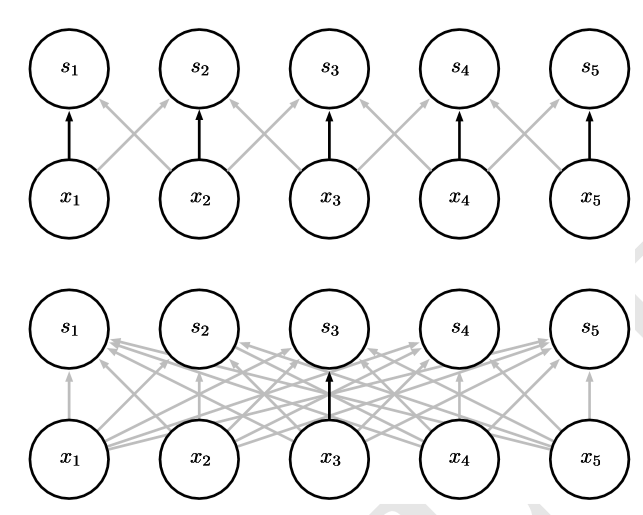
\includegraphics[width=0.4\textwidth]{graphic/cnn1.png}
\caption{CNN与ANN对比\cite{deeplearning2016} \label{cnn1}}
\end{center}
\end{figure}

\subsubsection{池化}
池化(Pooling)是卷积神经网络中非常重要的操作,能帮助学习输入特征的不变性,也能减少特征数量,增加计算速度。常见的池化方式有两种,最大池化和平均池化。最大池化给出了卷积层输出中一个矩形区域内特征的最大值,而平均池化则为矩形区域内特征的平均值。池化相当于简单使用某一位置附近区域的总体输出来代替各单元的输出。在自然语言处理中,最大池化的作用往往要好于平均池化,因此,本文采用最大池化方式。
\subsection{C\& W模型}
C\& W模型是由collobert等于2011年\cite{collobert2011} 提出的基于卷积神经网络的自然语言处理框架,该模型被设计能够适用于几乎所有自然语言处理任务,同时也能对某个任务进行细化以提高精度。C\& W模型分为两种模式,单词窗口和语句模式,后者主要结构如图\ref{candw1}。模型可以分为七层,输入层,查表层,卷积层,池化层,线性层和对应的激活函数层,最后是输出层。C\& W模型在各任务上都表现良好,接近为特定任务特化的系统性能,因此本文选择C\& W模型作为基本框架。
\begin{figure}
\begin{center}
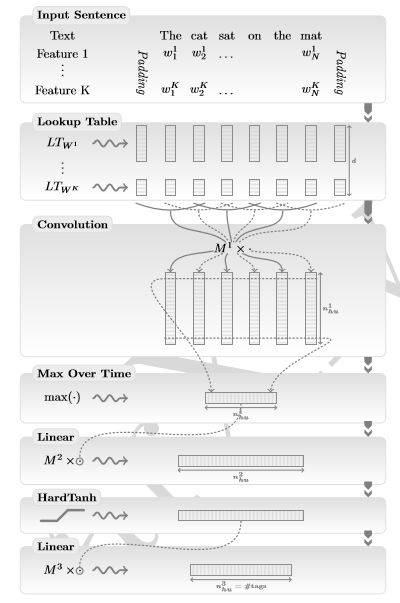
\includegraphics{graphic/candw1.png}
\caption{c\&w语句模式基本模型 \label{candw1}}
\end{center}
\end{figure}
\subsection{循环神经网络}
循环神经网络(Recurrent Neural Network)是专门用于处理序列数据的神经网络。如图,传统神经网络为序列中的每个状态分别训练权重,但RNN在时间步内共享参数。给定时间t的变量后,t+1时变量的条件概率分布是平稳的,不依赖于t,也即RNN具有时间上的平移不变性。\par
对于长度为{t}的序列$\vec{x}$,一般神经网络计算方式可以表示为:
\begin{equation}
h_t = g_t(x_t, x_{t-1},...,x_0;\theta)
\end{equation}
其中$\theta$代表所有网络参数。\par
而RNN的计算方式可以表示为:
\begin{equation}
h_t = g_t(x_t, x_{t-1},...,x_0;\theta) = f(h_{t-1}, x_t;\theta)
\end{equation}
RNN能将长度为t的序列映射为固定长度的向量,但这种映射通常是有损的,因此,需要保证$h_t$足够丰富,能够记住序列中的信息。
RNN主要有三种结构,a中每个时间步都有输出,并且隐藏单元与过去隐藏单元相关联,b中隐藏单元与过去输出相关联,而c中只有最后一个时间步有输出。由于语句级情感分析任务最终只有一个输出,所以本章中RNN结构符合c。
训练中,RNN使用通过时间反向传播算法(BPTT)反向推导t步梯度。实践中,为了降低复杂度,同时也因为梯度爆炸和梯度消失的限制,t往往取较小的定值。
\begin{center}
\begin{figure}
\subfigure{
	\label{fig:rnn1}
	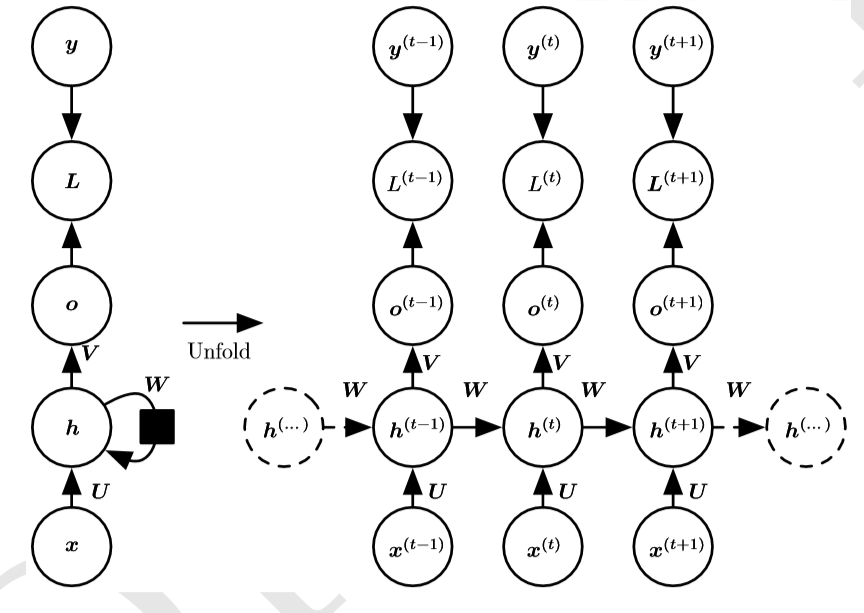
\includegraphics[width=0.3\textwidth]{graphic/rnn1.PNG}
}
\subfigure{
	\label{fig:rnn2}
	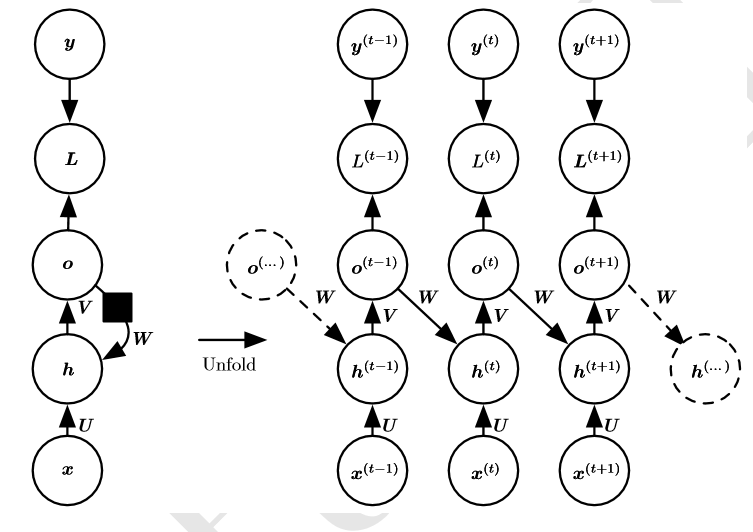
\includegraphics[width=0.3\textwidth]{graphic/rnn2.PNG}
}
\subfigure{
	\label{fig:rnn3}
	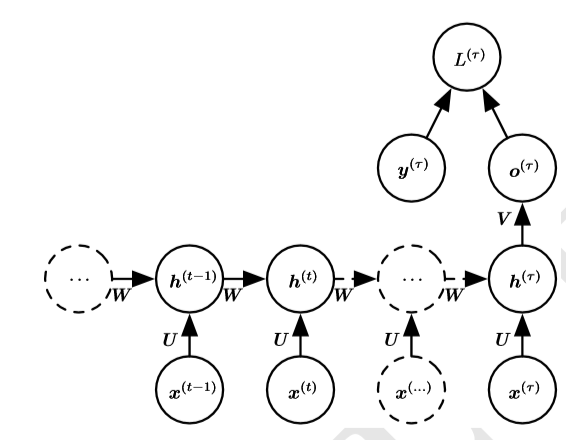
\includegraphics[width=0.3\textwidth]{graphic/rnn3.PNG}
}
\caption{RNN基本结构}
\end{figure}
\end{center}

\subsection{LSTM}
RNN为信息的持久化提供了行之有效的方法,但RNN存在梯度爆炸或梯度消失的问题。\par
考虑最简单的RNN单元,即:
\begin{equation}
h_t = W^Th_{t-1}
\end{equation}
该公式相当于:
\begin{equation}
h_t = {W^t}^Th_0
\end{equation}
若W符合下列形式的特征分解:
\begin{equation}
W=Q\Lambda Q^T
\end{equation}
则原式可以转化为:
\begin{equation}
h_t = Q^T\Lambda ^t Qh_0
\end{equation}
因此,$h_t$随时间成指数形式增长,若幅值小于1时,$h_t$将随t的增长趋向于0,出现梯度消失现象,而当幅值大于1时,$h_t$又激增,导致梯度爆炸。\par
为了减轻梯度消失问题,Hochreiter等\cite{lstm1997}提出了LSTM模型,该模型主要由以下四部分构成:
\begin{enumerate}
\item 遗忘门:控制状态更新
\item 输入门:控制信息保存。
\item 输出门:控制读取信息。
\item 记忆单元:存储状态。
\end{enumerate}
LSTM的具体计算流程如下:
\begin{equation}
i_t = \sigma(W_i  [h_{t-1},x_t] + b_i)
\end{equation}
其中$i_t$为输入门输出的结果,$W_i$为输入门的参数,$h_{t-1}$为上一时刻的输出,$x_t$为本时刻的输入,$b_i$为输入门的参数偏置。
\begin{equation}
u_t = \tanh{(W_u [h_{t-1},x_t] + b_u)}
\end{equation}
其中$u_t$为记忆单元得到的结果,$W_u$为记忆单元的参数,$b_u$为输入门的参数偏置。
\begin{equation}
f_t = \sigma{(W_f [h_{t-1},x_t] + b_f)}
\end{equation}
其中$f_t$为遗忘门输出的结果,$W_f$为遗忘门的参数,$b_f$为遗忘门的参数偏置。
\begin{equation}
C_t = f_t C_{t-1} + i_t \times u_t
\end{equation}
其中$C_t$为本时间点的状态。
\begin{equation}
o_t = \sigma{(W_o [h_{t-1},x_t] + b_o)}
\end{equation}
其中$o_t$为输出门输出的结果,$W_o$为输出门的参数,$b_o$为输出门的参数偏置。
\begin{equation}
h_t = o_t \times tanh{(C_t)}
\end{equation}
其中$h_t$为最终输出结果。
\begin{figure}[!hbp]
\begin{center}
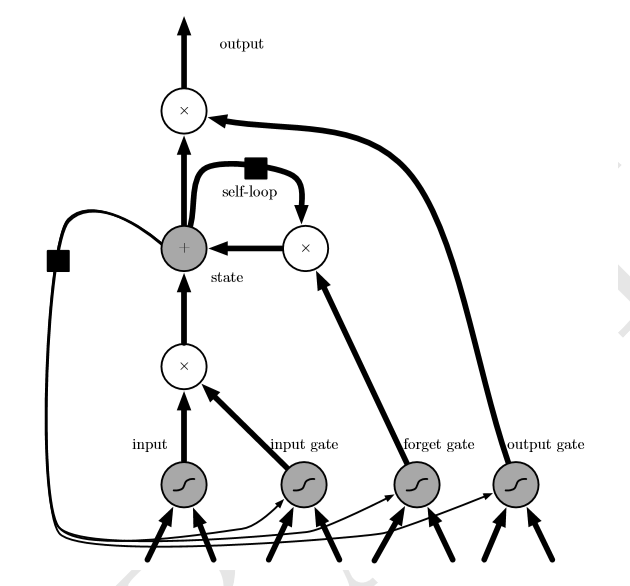
\includegraphics[width=0.4\textwidth]{graphic/lstm1.png}
\caption{LSTM基本结构\cite{deeplearning2016} \label{lstm1}}
\end{center}
\end{figure}